% Tipo de documento: artículo.
\documentclass[11pt, a4paper]{article}

% Podemos poner "titlepage" como opción
% para que el título esté en una página separada, por ejemplo:
% \documentclass[11pt, a4paper, titlepage]{article}

%% Algunos paquetes adicionales.

% Cadenas traducidas al español.
\usepackage[spanish, es-tabla,es-noquoting,es-noshorthands]{babel}

% Para poder poner acentos, ñ's y similares en el documento.
\usepackage[T1]{fontenc}
\usepackage[utf8x]{inputenc}

% Paquetes para matemáticas
\usepackage{amsthm}
\usepackage{amsmath}
\usepackage{amssymb}

\usepackage{tikz} 		% Dibujos
\usepackage{listings} 	% Ejemplos de código
\usepackage{hyperref} 	% Enlaces

% Interesante: Probar a cambiar el color de los enlaces.
\hypersetup{
	hyperindex,
	colorlinks,
	allcolors = blue!50!black
}

% Interesante: Ver qué pasa si se cambian estas longitudes
\setlength{\parskip}{0pt}
\setlength{\parindent}{10pt}

% Título, autor y fecha
\title{Un documento de muestra}
\author{Un autor}
\date{\today}

\begin{document}

\maketitle

% Interesante: Cambiar la profundidad de secciones que aparecen en la tabla de contenidos.
\setcounter{tocdepth}{2}

\tableofcontents

\section{Una sección}

% Básico: Probar a cambiar el formato de este párrafo: poner negritas, cambiar de color o cambiar de tamaño.
Un párrafo en el que podemos escribir cosas, y ver cómo queda. Un ejercicio interesante: cambiar el formato del párrafo. Por ejemplo, ponerlo en color azul, o reducir el tamaño de letra.

% Básico: probar el efecto de poner // y ver cómo queda (Spoiler: mal).
A modo de recordatorio,
cambiar de línea
no cambia de párrafo.

\subsection{Una subsección}

\subsubsection{Una subsubsección}

\section*{Sección sin número}

% Básico: probar a cambiar la cadena hbtp y ver dónde queda la imagen
\begin{figure}[hbtp]
\centering
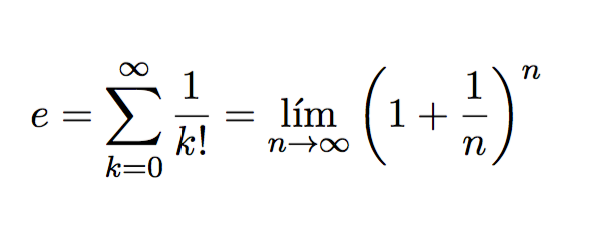
\includegraphics[width = 0.4\textwidth]{Ecuacion.png}
\caption{¿Cómo se podría escribir esta ecuación en \LaTeX?}
\label{fig:ecuacion}
\end{figure}

% Básico: tratar de escribir la ecuación de la figura anterior
\[ e = ... \]

% Interesante: Tratar de arreglar esta ecuación para que salga bien.
% Es recomendable usar caracteres de espaciado (\, o \;) y comandos de texto
\[ f continua en x_0 \iff \forall \epsilon > 0 \exists \delta > 0 tal que |x - x_0| < \delta \implies |f(x) - f(x_0)| < \epsilon \]

% Básico: Probar a cambiar de align a multline o gather para ver cómo queda
% Nota: Acordaos de quitar los & que marcan la alineación, si no fallará.
\begin{align*} I^2 &=
	\left(\int_{\mathbb{R}} e^{-x^2} \mathrm{d}x\right)^2 \\
	&= \iint_{\mathbb{R}^2} e^{-(x^2+y^2)} \mathrm{d}x \mathrm{d}y \\
	&= \int_0^{2\pi} \int_{0}^\infty e^{-r^2} r\, \mathrm{d} r \mathrm{d} \theta = \\
	&= 2 \pi \int_{0}^\infty e^{-r^2} r\, \mathrm{d} r = \\
	&= \pi \left(e^{-r^2}\right|_{r = 0}^{\infty} = \\
	&= \pi
\end{align*}

\end{document}
